\documentclass[ngerman,compress,hyperref={bookmarks}]{beamer}
\usetheme{Antibes}
\useoutertheme{infolines}
\usepackage[utf8x]{inputenc}

\usepackage{multirow}

\usepackage{colortbl}
\definecolor{dunkelgrau}{rgb}{0.8, 0.8, 0.8}

\usepackage{wasysym}

\logo{
\includegraphics[height=1cm]{images/logoHAW}}
\usepackage{graphicx}
%\usepackage[%
%	bibstyle=authoryear,%
%	citestyle=authoryear,%
%	bibencoding=utf8,%
%	bibtex8=true,%
%	sorting=nyt,%
%	sortcites=true,%
%	maxnames=2,%
%	babel=other,%
%	block=space,%
%	backref=false,%
%	natbib=true,%
%	hyperref=true,%
%]{biblatex}
%\bibhang1em
%\usepackage[style=authortitle-icomp]{biblatex}
%\bibliography{routing_atlas}

%\setbeamertemplate{bibliography entry title}{}
%\setbeamertemplate{bibliography entry location}{}

\title{Aktive Messverfahren zur Topologievalidierung\\ im Routing-Atlas}
\subtitle{Vortrag: Ringvorlesung Seminar}
\subject{Routing-Atlas, Topology}
\author{Andreas Krohn}
\institute[HAW]{Hochschule für Angewandte Wissenschaften Hamburg}
\date[WS 2012/13]{14. November 2012}

\begin{document}
\frame[plain]{\titlepage}

\section*{Agenda}
\begin{frame}{Agenda} \setcounter{tocdepth}{1} \tableofcontents[part=1] \setcounter{tocdepth}{3} \end{frame}

\part{Hauptteil}
\section{Intro}

\subsection{Routing-Atlas}
\begin{frame}[allowframebreaks]{Routing-Atlas}
\nocite{wsbh-envgi-12}
\nocite{Faloutsos:1999:PRI:316194.316229}
\nocite{Dimitropoulos:2007:RIV:1198255.1198259}
\nocite{0903.3218v1}
  \begin{itemize}
    \item Projekt der inet AG und des BSI
    \item Topologieanalyse um landesspezifische Teile des Internets zu
    \begin{itemize}
      \item Identifizieren
      \item Klassifizieren
      \item Visualisieren
    \end{itemize}
  \end{itemize}
  \vspace{0.1cm}
  {\small
  \begin{thebibliography}{}
    \bibitem{wsbh-envgi-12} ``Exposing a Nation-Centric View on the German Internet – A Change in Perspective on the AS Level''
    \newblock Matthias Wählisch, Thomas C. Schmidt, Markus de Brün, Thomas Häberlen\\
    \newblock In Proc. of the 13th Passive and Active Measurement Conference (PAM), volume 7192 of LNCS, page 200–210, Berlin Heidelberg, 2012. Springer-Verlag.\\[-20pt]
  \end{thebibliography}
  %\url{http://inet.cpt.haw-hamburg.de/projects/routing-atlas/}
  }
  \framebreak
% \end{frame}
%
% \subsection{Bestandteile des Routingatlas}
% \begin{frame}[allowframebreaks]{Bestandteile des Routingatlas}
  \begin{enumerate}
  \item Identifikation deutscher Autonomer Systeme
  \begin {itemize}
    \item IP-Blöcke identifizieren
    \item Zu IP-Präfixen auflösen
    \item IP-Päfixe Autonomen Systemen zuordnen
  \end{itemize}
  \item Neu dazugekommen: Validierung mittels Maxmind \& Cymru
  \item Klassifikation Autonomer Systeme
  \begin{itemize}
    \item Topologische Einordnung
    \item Branchen
  \end{itemize}
  \item Routing-Graphen bilden
  \begin{itemize}
    \item Routing Matrix des NEC-Lab
  \end{itemize}
  \framebreak
  \item Visualisierung der (Teil)Graphen
  \end{enumerate}

  \begin{columns}[c]
    \begin{column}{0.5\textwidth}
      \begin{figure}
        \label{asgraphs}
        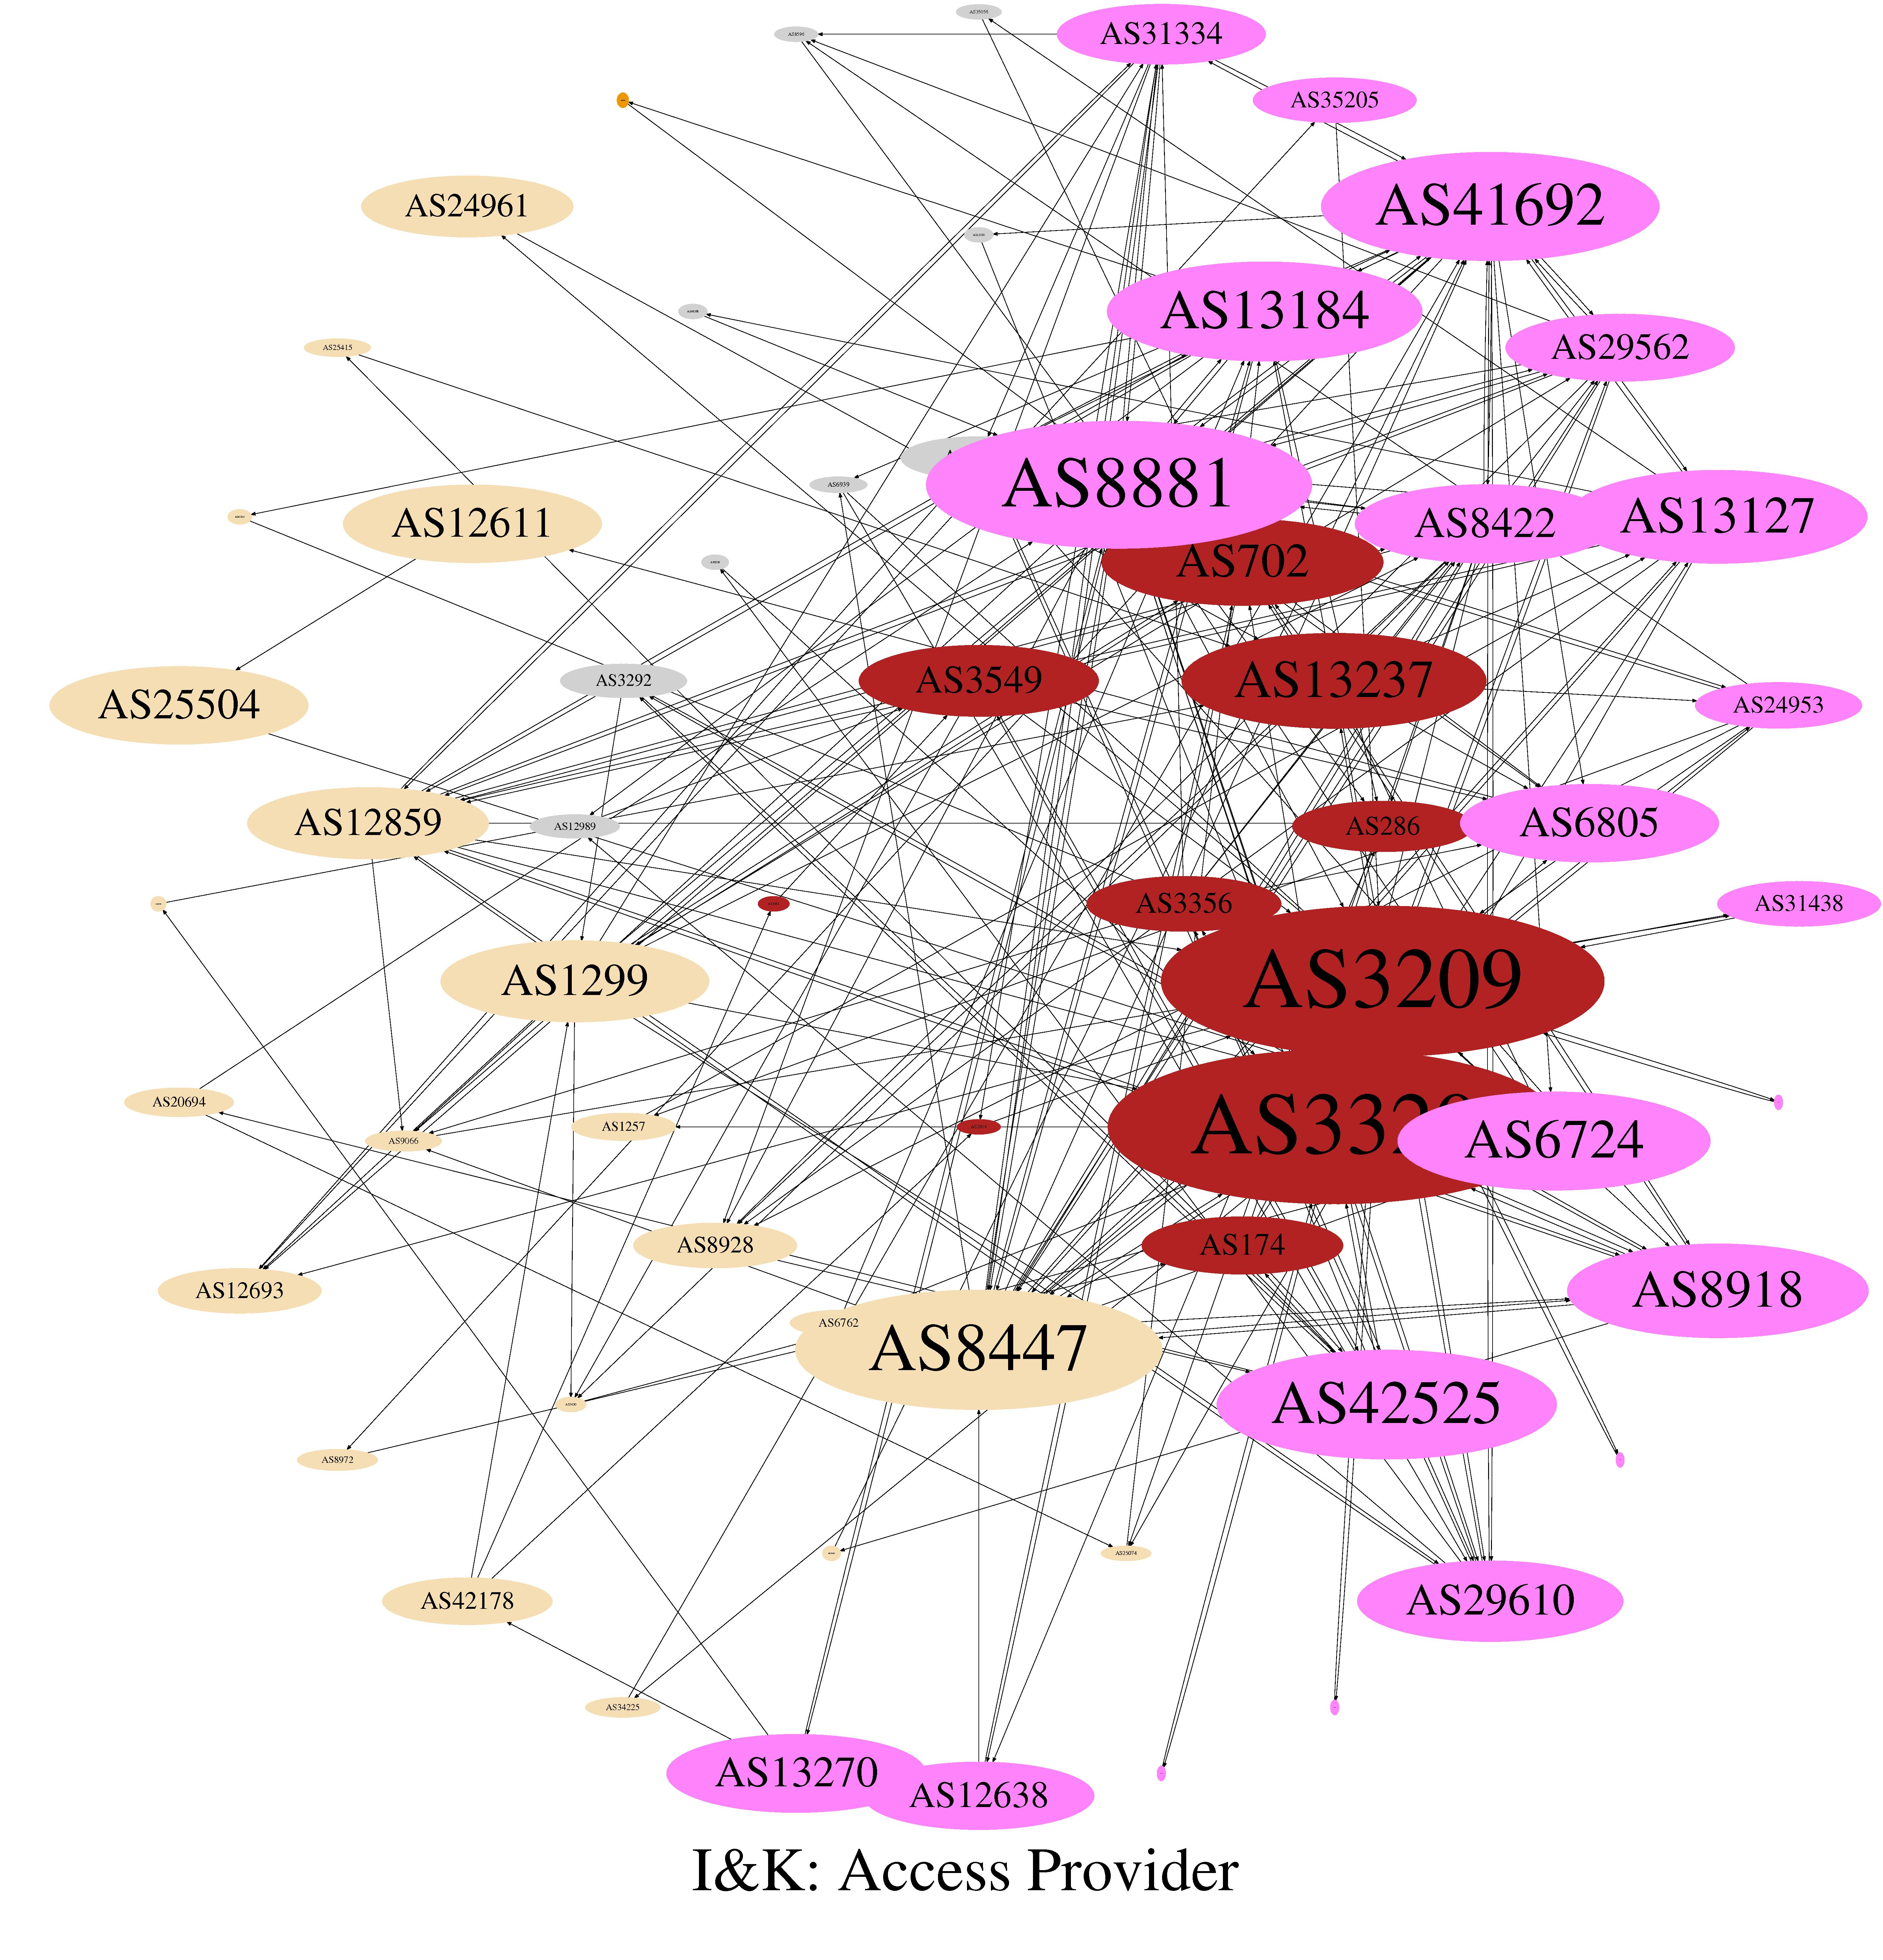
\includegraphics[width=1\textwidth]{images/asgraph_cat5-pos-betweenness}
      \end{figure}
    \end{column}
    \begin{column}{0.5\textwidth}
      \begin{figure}
        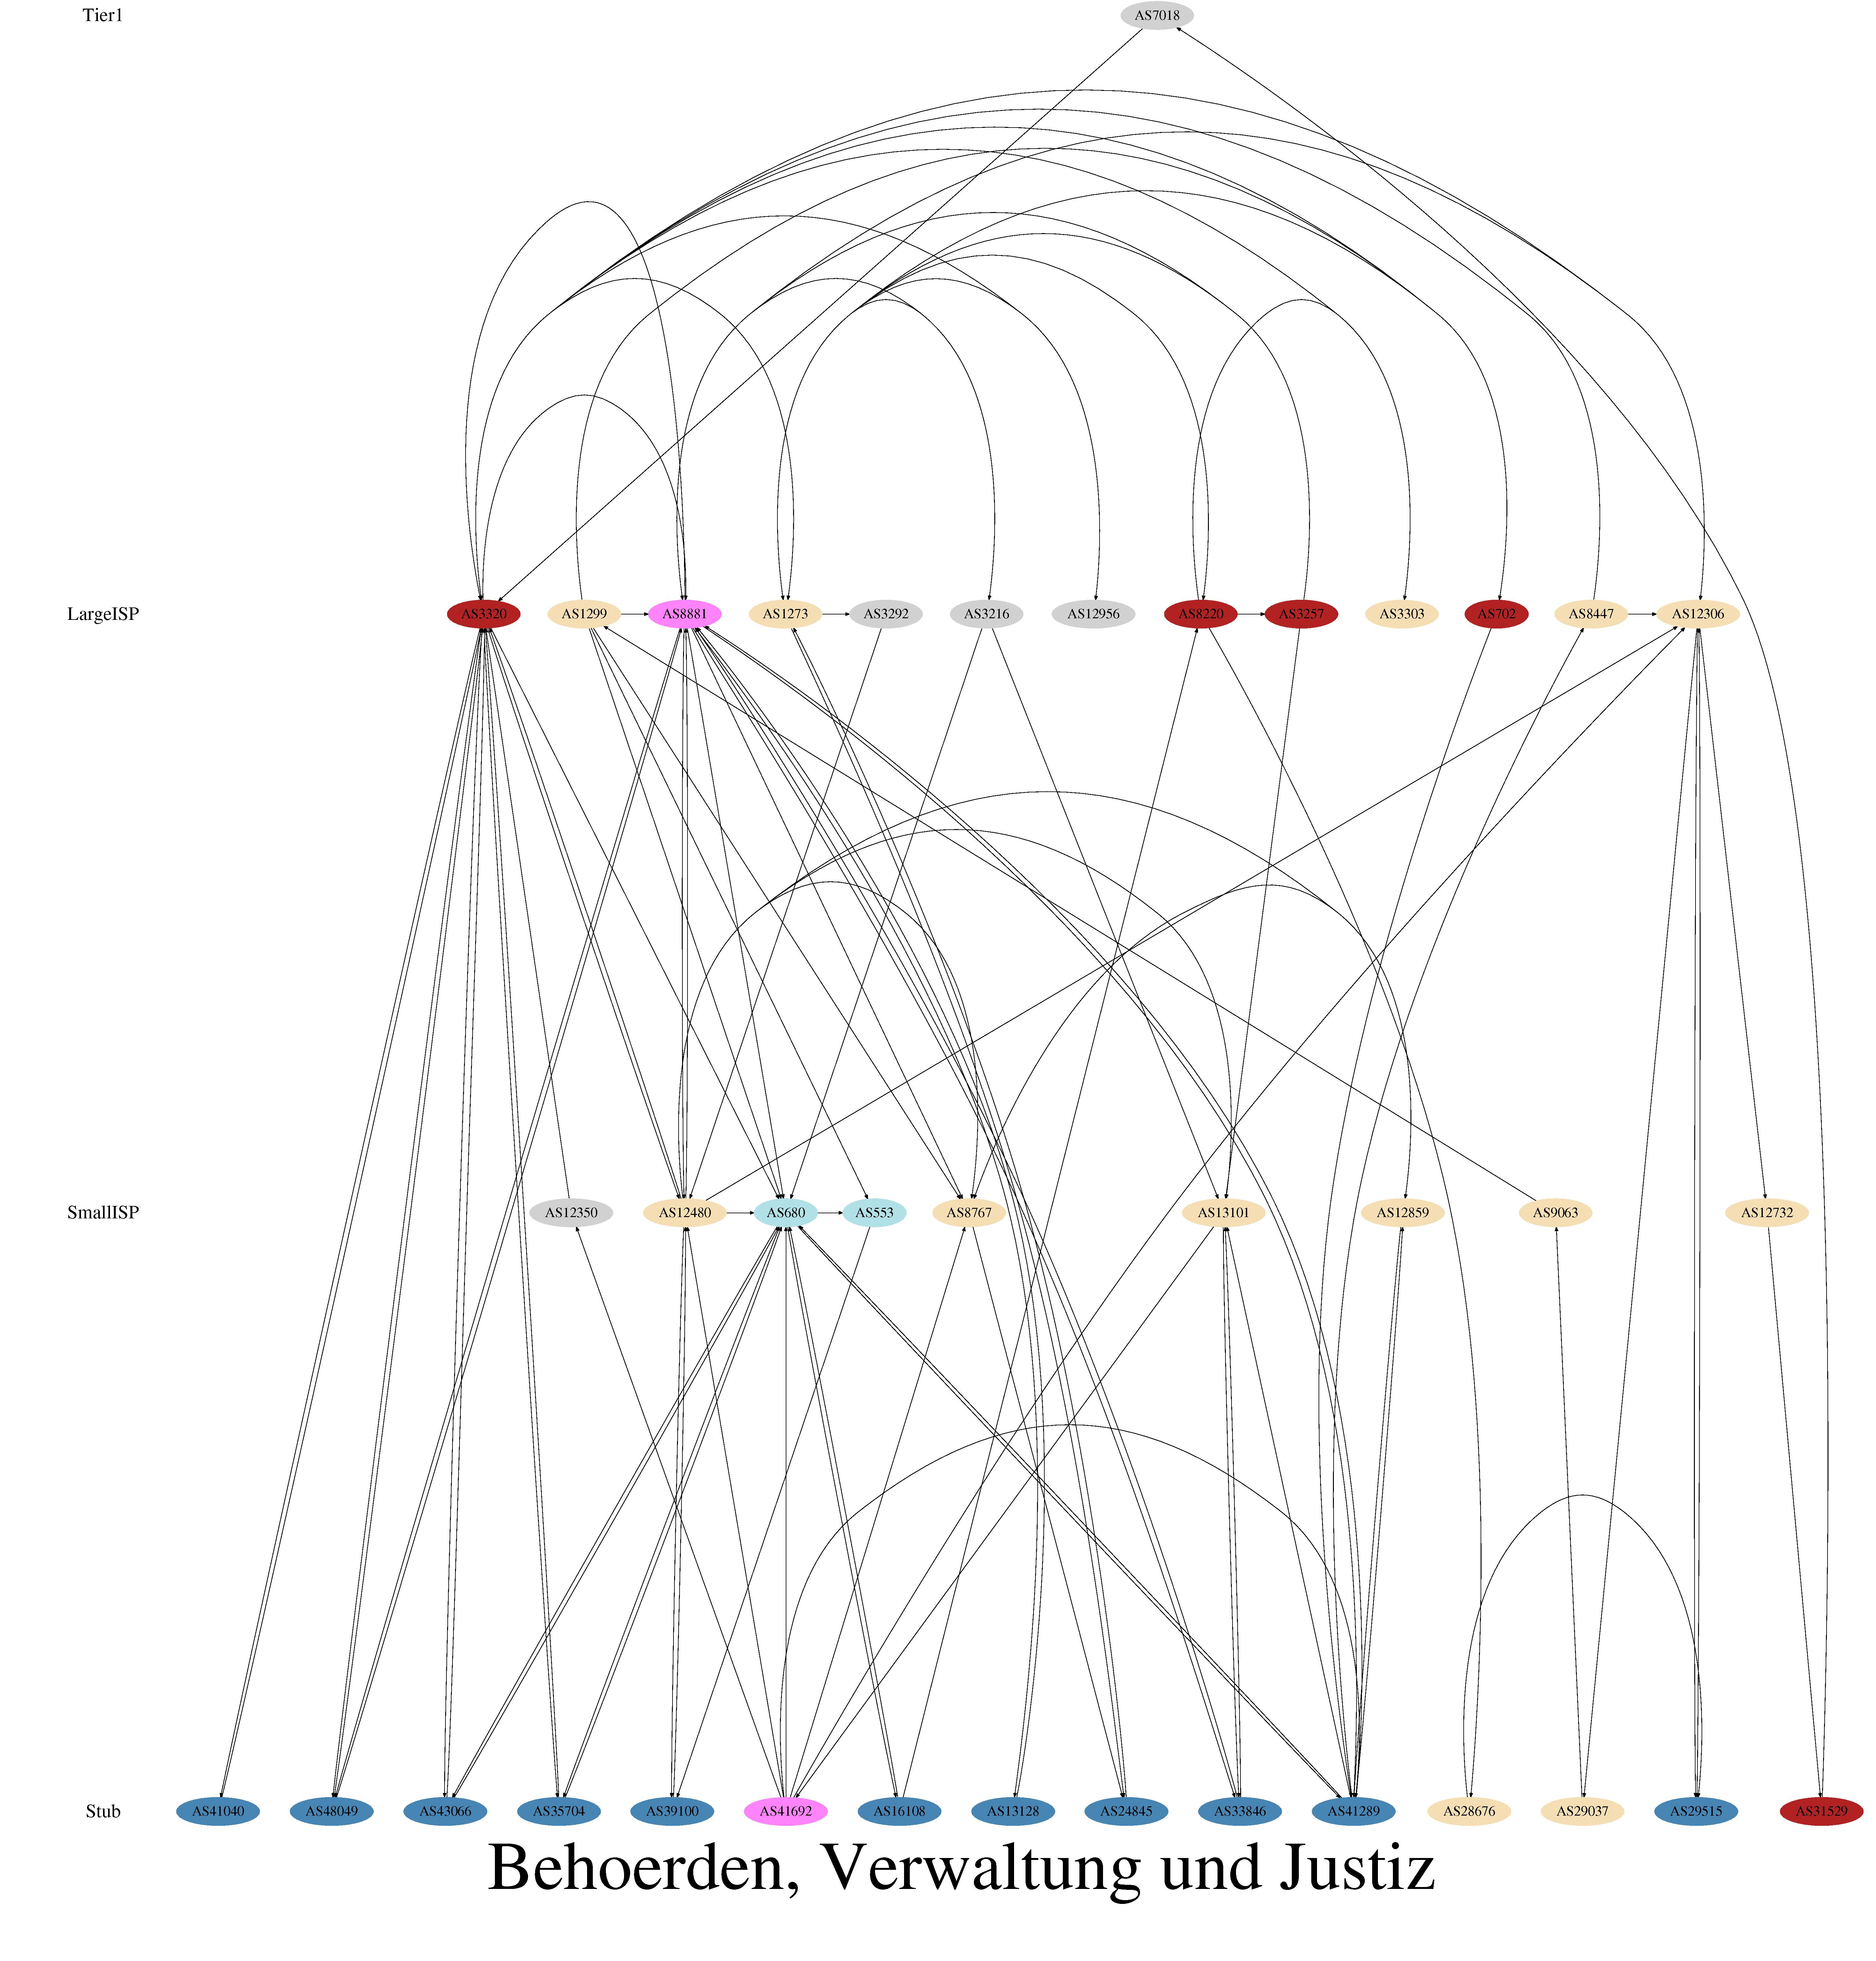
\includegraphics[width=1\textwidth]{images/asgraph_cat9-dot}
      \end{figure}
    \end{column}
  \end{columns}
\end{frame}



\subsection{Ziel}
\begin{frame}{Ziel}
  \begin{center}
    {\Large Erweiterung des Routing-Atlas}\\
    \vspace{0.5cm}
    Routing Matrix ersetzen\\
    \vspace{0.5cm}
    Dazu:
    \begin{itemize}
      \item Datenquellen evaluieren\\{\scriptsize(Routingtabellen, BGP Peering Informationen der IRR, UCLA-Daten, \ldots)}
      \item Heuristik zur Bewertung von Inter-AS Links\\{\scriptsize(Policy basiertes Routing nachbilden)}
      \item Routing Matrix berechnen
    \end{itemize}
  \end{center}
\end{frame}

% \section*{Agenda}
% \begin{frame}{Agenda} \setcounter{tocdepth}{1} \tableofcontents[part=1] \setcounter{tocdepth}{3} \end{frame}

\section{Datenquellen}
\subsection{Grundlagen, Problemstellung}
\begin{frame}{Datenquellen}{Grundlagen, Problemstellung}
  \begin{itemize}
    \item Internet: Ansammlung Autonomer Systeme
    \item Routingbeziehungen nicht zentral erfasst\\$\rightarrow$ also: Messen, Sammeln
  \end{itemize}

  \begin{columns}[t]
    \begin{column}{0.4\textwidth}
      passiv
      \begin{itemize}
        \item BGP trace collectors\\{\scriptsize z.B. RouteViews, RIPE RIS}
        \item Öffentlich zugängliche Router
        \item Internet Routing Registries\\{\scriptsize z.B. RIPE}
      \end{itemize}
    \end{column}
    \begin{column}{0.4\textwidth}
      aktiv
      \begin{itemize}
        \item traceroute
      \end{itemize}
    \end{column}
  \end{columns}
\end{frame}

\subsection{Related Work, Zhang et al}
\begin{frame}{Collection the Internet AS-level Topology\footnote{\url{http://irl.cs.ucla.edu/topology/}}}{2005, \cite{Zhang:2005:CIA:1052812.1052825}}
  \begin{columns}[c]
    \begin{column}{0.5\textwidth}
      ``most complete AS-level topology''
      \begin{itemize}
        \item Verfügbare Daten sammeln
        \item Konsistenzchecks\\{\scriptsize Manuelle gepflegte IRR Einträge}
        \item Normalisierung
        \item Einordnung von ASen und Links
        \item Tägliche Veröffentlichung
      \end{itemize}
      \vspace{1cm}
    \end{column}
    \begin{column}{0.08\textwidth}
      \begin{figure}
        \label{zhang_et_al}
        \includegraphics[width=1\textwidth]{images/zhang_b}\\
        \includegraphics[width=1\textwidth]{images/person}\\
        \includegraphics[width=1\textwidth]{images/massey}\\
        \includegraphics[width=1\textwidth]{images/zhang_l}
      \end{figure}
    \end{column}
    \begin{column}{0.3\textwidth}
      {\scriptsize Beichuan Zhang\\
      \vspace{0.1cm}
      UCLA\\
      \vspace{0.7cm}
      Raymond Liu\\
      \vspace{0.1cm}
      UCLA\\
      \vspace{0.3cm}
      Daniel Massey\\
      \vspace{0.1cm}
      Colorado State University\\
      \vspace{0.3cm}
      Lixia Zhang\\
      \vspace{0.1cm}
      UCLA\\ }
    \end{column}
  \end{columns}
\end{frame}

\subsection{Related Work, Augustin et al}
\begin{frame}{IXPs: Mapped?\footnote{\url{http://www-rp.lip6.fr/~augustin/ixp/}}}{2009, \cite{Augustin:2009:IM:1644893.1644934}}
  \begin{columns}[c]
    \begin{column}{0.55\textwidth}
      \begin{itemize}
        \item IXPs, Mitglieder und Präfixe
        \item Looking Glass Server in ASen der Mitglieder
        \item traceroutes "durch" die IXPs
      \end{itemize}
      \begin{figure}
        \label{augustin_ixp}
        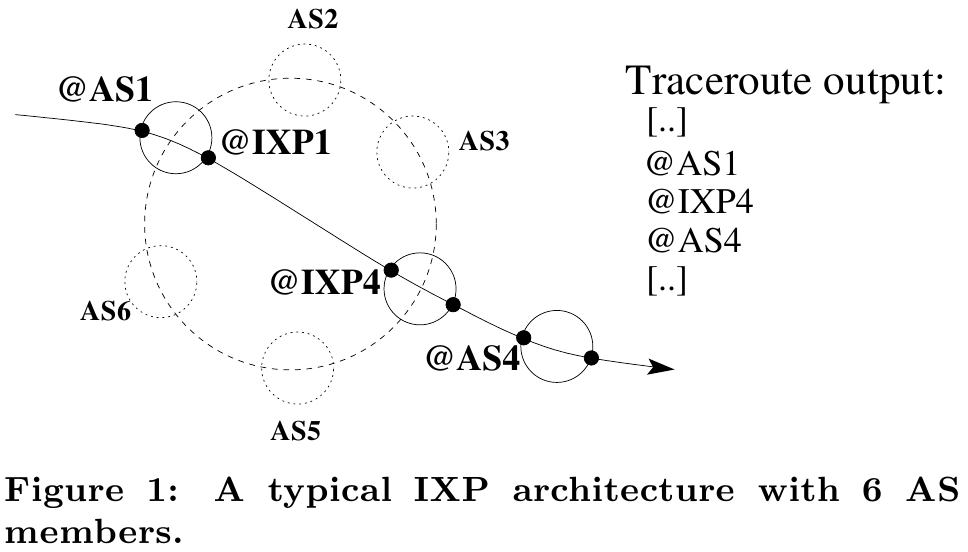
\includegraphics[width=1\textwidth]{images/augustin_ixp}
      \end{figure}
    \end{column}
    \begin{column}{0.1\textwidth}
      \begin{figure}
        \label{augustin}
        \includegraphics[width=1\textwidth]{images/augustin_b}\\
        \includegraphics[width=1\textwidth]{images/krishnamurthy_b}\\
        \includegraphics[width=1\textwidth]{images/willinger_w}
      \end{figure}
    \end{column}
    \begin{column}{0.3\textwidth}
      {\scriptsize Brice Augustin\\
      \vspace{0.1cm}
      Université Pierre et Marie Curie, Paris\\
      \vspace{0.5cm}
      Balachander Krishnamurthy\\
      \vspace{0.1cm}
      AT\&T Labs-Research, Floham Park\\
      \vspace{0.3cm}
      Walter Willinger\\
      \vspace{0.1cm}
      AT\&T Labs-Research, Floham Park\\ }
    \end{column}
  \end{columns}
\end{frame}

% achivement: ein Haufen AS-Links/AS-Pfade

\section{Modellierung}

\subsection{Grundlagen}
\begin{frame}{Modellierung}{Grundlagen}
  \begin{columns}[c]
    \begin{column}{0.7\textwidth}
      \begin{itemize}
        \item AS Hierarchie
        \item Routingbeziehung zwischen ASen $\rightarrow$ AS-Link
      \end{itemize}
      \begin{description}
        \item[C2P] Customer zahlt für Transit (a)
        \item[Peering] kostenneutraler Trafficaustausch (b)\\{\scriptsize (meist) kein Transit}
        \item[Sibling] kostenneutraler Transit (c)\\{\scriptsize z.B. mehrere ASe eines Konzerns}
      \end{description}
    \end{column}
    \begin{column}{0.3\textwidth}
      \begin{figure}
        \includegraphics[width=1\textwidth]{images/Routingbeziehungen}
      \end{figure}
    \end{column}
  \end{columns}
\end{frame}

\subsection{Problemstellung}
\begin{frame}{Problemstellung}
  \begin{figure}
    \includegraphics[width=0.75\textwidth]{images/Topologyinference}
  \end{figure}
\end{frame}


%\section{AS-Beziehungen, valley-free routing}
%\begin{frame}{AS-Beziehungen, valley-free routing}
% \begin{columns}[c]
%  \begin{column}{0.2\textwidth}
%  \end{column}
%  \begin{column}{0.5\textwidth}
%    \begin{enumerate}
%     \item[customer-provier] customer zahlt für Transit
%     \item[peering] kostenloser Trafficaustausch
%     \item[sibling] kostenloser Transit\\ \vspace{0.5cm}
%     \item[valley-free routing] Transit nur über ``höhere'' ASes
%    \end{enumerate}
%  \end{column}
%  \begin{column}{0.3\textwidth}
%   \begin{figure}
%    \label{asrelations}
%    \includegraphics[width=1\textwidth]{images/asrelation}
%   \end{figure}
%    {\scriptsize }
%  \end{column}
% \end{columns}
%\end{frame}

\subsection{Related Work, Gao}
\begin{frame}{On Inferring Autonomous System Relationships in the Internet}{2001, \cite{Gao:2001:IAS:504611.504616}}
  \begin{columns}[c]
    \begin{column}{0.5\textwidth}
      \begin{itemize}
        \item connectivity vs. reachability
        \item AS Pfade aus BGP Routing Tabellen
        \item Knotengrad als Heuristik
        \item Einordnung in C2P, Peering, Sibling
        \item Valley-free Routing
      \end{itemize}
    \end{column}
    \begin{column}{0.1\textwidth}
      \begin{figure}
        \includegraphics[width=1\textwidth]{images/gao}
        \label{gao}
      \end{figure}
    \end{column}
    \begin{column}{0.3\textwidth}
      {\scriptsize Lixin Gao\\
      \vspace{0.1cm}
      University of Massachusetts\\
      AT\&T Research Labs\\}
    \end{column}
  \end{columns}
\end{frame}

% \subsection{Related Work, Karlin et al}
% \begin{frame}{Nation-State Routing: Censorship, Wiretapping, and BGP}{2009, \cite{0903.3218v1}}
%   \begin{columns}[c]
%     \begin{column}{0.5\textwidth}
%       \begin{itemize}
%         \item Zuordnung IP-Präfix zu Land
%         \item ...
%       \end{itemize}
%     \end{column}
%     \begin{column}{0.09\textwidth}
%       \begin{figure}
%         \label{karlin}
%         \includegraphics[width=1\textwidth]{images/karlin_j}\\
%         \includegraphics[width=1\textwidth]{images/forrest_s}\\
%         \includegraphics[width=1\textwidth]{images/rexford_j}
%       \end{figure}
%     \end{column}
%     \begin{column}{0.3\textwidth}
%       {\scriptsize Josh Karlin\\
%       \vspace{0.1cm}
%       University of New Mexico\\
%       \vspace{0.7cm}
%       Stephanie Forrest\\
%       \vspace{0.1cm}
%       University of New Mexico\\
%       \vspace{0.5cm}
%       Jennifer Rexford\\
%       \vspace{0.1cm}
%       Princeton University\\ }
%     \end{column}
%   \end{columns}
% \end{frame}

\subsection{Related Work, Winter}
\begin{frame}{Modeling the Internet Routing Topology - In Less than 24h}{2009, \cite{Winter:2009:MIR:1577959.1577976}}
  \begin{columns}[c]
    \begin{column}{0.5\textwidth}
      \begin{itemize}
        \item Präfix vs. AS Graph
        \item AS-Links aus den UCLA Daten\\{\scriptsize{(s. Folie \pageref{zhang_et_al})}}
        \item Bewertung der Links
        \item Routing Matrix berechnen
      \end{itemize}
      {\small
      \begin{itemize}
        \item Routing Matrix ist eine der Datenquellen für den Routing-Atlas
        \item Projekt leider eingestellt
      \end{itemize}}
    \end{column}
    \begin{column}{0.09\textwidth}
      \begin{figure}
        \label{winter}
        \includegraphics[width=1\textwidth]{images/winter_r}
      \end{figure}
    \end{column}
    \begin{column}{0.3\textwidth}
      {\scriptsize Rolf Winter\\
      \vspace{0.2cm}
      NEC Labs Europe\\jetzt: Hochschule Augsburg\\}
    \end{column}
  \end{columns}
\end{frame}


\section{Ausblick}
\begin{frame}{Ausblick}
  \begin{itemize}
    \item Projekt 1
    \begin{itemize}
      \item Routing Matrix aktualisieren
    \end{itemize}
    \item Später..
    \begin{itemize}
      \item Weitere Datenquellen (IXPs, Peering, \ldots)
      \item Regelmäßige Veröffentlichung aktueller Daten
      \item Peeroskop
    \end{itemize}
  \end{itemize}
% \begin{itemize}
%  \item Aktuelle shortest path matrix
%  \begin{itemize}
%   \item Topologieänderungen
%  \end{itemize}\vspace{1cm}
%  \item Andere Länder, Visualisierungen, Online-Tool, IPv6
%  \begin{itemize}
%   \item Breiteres Publikum
%   \item Zukunftsfähigkeit
%  \end{itemize}
% \end{itemize}
\end{frame}


% \begin{frame}{On power-law relationships of the Internet topology}{1999, \cite{Faloutsos:1999:PRI:316194.316229}}
%   \begin{columns}[c]
%     \begin{column}{0.5\textwidth}
%       \begin{itemize}
%         \item Graphentheoretische Betrachtung der Inter- \& Intradomain Topologie
%         \item Entdeckung exponentieller Zusammenhänge zwischen
%         \begin{itemize}
%           \item ausgehenden Links und Rang eines AS
%           \item Häufigkeit und Anzahl ausgehender Links
%           \item Eigen exponent?
%         \end{itemize}
%       \end{itemize}
%     \end{column}
%     \begin{column}{0.1\textwidth}
%       \begin{figure}
%         \includegraphics[width=1\textwidth]{images/faloutsos_m}\\
%         \includegraphics[width=1\textwidth]{images/faloutsos_p}\\
%         \includegraphics[width=1\textwidth]{images/faloutsos_c}
%         \label{faloutsos}
%       \end{figure}
%     \end{column}
%     \begin{column}{0.3\textwidth}
%       {\scriptsize Micalis Faloutsos\\
%       \vspace{0.1cm}
%       University of California\\
%       \vspace{0.8cm}
%       Petros Faloutsos\\
%       \vspace{0.1cm}
%       University of Toronto\\
%       \vspace{0.7cm}
%       Christos Faloutsos\\
%       \vspace{0.1cm}
%       Carnegie Mellon University\\ }
%     \end{column}
%   \end{columns}
% \end{frame}

\part{Ende}
\subsection{kthxbye}
\begin{frame}[plain]{Ende}
\begin{columns}[t]
\begin{column}{0.5\textwidth}
 \begin{center}
 \vspace{1cm}
 Vielen Dank für die Aufmerksamkeit\\
 \vspace{1.5cm}
 Fragen\ldots?
 \end{center}
\end{column}
\begin{column}{0.5\textwidth}
 \vspace{-1cm}
 \begin{figure}
  \label{asngraphs2}
  \includegraphics[width=\textwidth]{images/asgraph_cat4-pos}
 \end{figure}
\end{column}
\end{columns}
\end{frame}

\section{Literatur}
\begin{frame}[plain, allowframebreaks]{Literatur}
\scriptsize
\bibliographystyle{alpha}
%\bibliographystyle{apalike}
\bibliography{folien}
\end{frame}

\section{Bildquellen}
\begin{frame}[plain]{Bildquellen}
  \scriptsize
%   \tiny
  \begin{table}
    \begin{tabular}{ c p{0.8\textwidth} }
      Seite & Quelle \\ \hline
      \pageref{asgraphs}, \pageref{asngraphs2} & \url{http://inet.cpt.haw-hamburg.de/projects/routing-atlas/}\\ \hline
%       & \multirow{3}{0.8\textwidth}{\url{http://www.cs.ucr.edu/~michalis/},\\ \url{http://www.cse.yorku.ca/cspeople/faculty/pfal/index.html},\\ \url{http://www.cs.cmu.edu/~christos/}} \\
%       \pageref{faloutsos}& \\
%       & \\ \hline
      & \multirow{3}{0.8\textwidth}{\url{http://www.cs.arizona.edu/~bzhang/},\\ \url{http://www.cs.colostate.edu/~massey/},\\ \url{http://www.cs.ucla.edu/~lixia/}} \\
      \pageref{zhang_et_al} & \\
      & \\ \hline
%       & \multirow{3}{0.8\textwidth}{\url{http://www.cs.unm.edu/~karlinjf/},\\ \url{http://www.cs.unm.edu/~forrest/},\\ \url{http://www.cs.princeton.edu/~jrex/}} \\
%       \pageref{karlin} & \\
%       & \\ \hline
      & \multirow{4}{0.8\textwidth}{\url{http://www-rp.lip6.fr/~augustin/},\\ \url{http://www.njit.edu/news/2011/2011-054.php},\\ \url{http://www.research.att.com/people/Willinger_Walter/index.html?fbid=Y-QjC_arIwn}} \\
      \pageref{augustin} (rechts) & \\
      & \\ & \\ \hline
      \pageref{augustin_ixp} (l. unten) & \url{http://www-rp.lip6.fr/~augustin/ixp/imc2009.pdf} \\ \hline
      \pageref{gao} & \url{http://www-unix.ecs.umass.edu/~lgao/} \\ \hline
      \pageref{winter} & \url{http://www.hs-augsburg.de/fakultaet/informatik/person/professor/winter_rolf/index.html} \\ \hline
    \end{tabular}
  \end{table}
\end{frame}

\end{document}
